% REV-ECIT 2026 — Tiểu ban AI và ứng dụng liên ngành.
% Quy cách: tiếng Việt, IEEE conference, A4, tối đa 6 trang.
% Bố cục bám theo bài mẫu cùng tiểu ban trong kỷ yếu REV-ECIT 2025 (tr. 331–336).
% Biên dịch: ./compile.sh (XeLaTeX, vì cần font có đủ dấu tiếng Việt).
\documentclass[conference,a4paper]{IEEEtran}

\usepackage{fontspec}
\setmainfont{texgyretermes}[
  Extension=.otf,
  UprightFont=*-regular, BoldFont=*-bold,
  ItalicFont=*-italic, BoldItalicFont=*-bolditalic]
\usepackage{cite}
\usepackage{amsmath,amssymb}
\usepackage{graphicx}
\usepackage{booktabs}
\usepackage{xcolor}
\usepackage{url}

\graphicspath{{figures/}}
\newcommand{\TBD}{\textcolor{red}{\textsc{tbd}}}
% Số liệu sinh bởi make_tables.py; chưa có thì mọi chỗ dùng macro vẫn dịch được.
\IfFileExists{generated/macros.tex}{% Generated by make_tables.py — do not edit.
\newcommand{\BloomKappa}{0.90}
\newcommand{\BloomN}{4219}
\newcommand{\ModelLabel}{Qwen3.5-2B}
\newcommand{\NScenCmp}{30}
\newcommand{\cmpAGAddie}{59.0}
\newcommand{\cmpAGAddieSD}{2.8}
\newcommand{\cmpAGTraj}{69.7}
\newcommand{\cmpAGTrajSD}{5.9}
\newcommand{\cmpAGTotal}{62.2}
\newcommand{\cmpAGTotalSD}{2.3}
\newcommand{\cmpAGTok}{282}
\newcommand{\cmpAGCalls}{70}
\newcommand{\cmpAGMin}{86}
\newcommand{\cmpEduAddie}{30.0}
\newcommand{\cmpEduAddieSD}{19.8}
\newcommand{\cmpEduAddieDiff}{28.9}
\newcommand{\cmpEduAddieP}{${<}\,0.001$}
\newcommand{\cmpEduTraj}{53.0}
\newcommand{\cmpEduTrajSD}{32.7}
\newcommand{\cmpEduTrajDiff}{16.6}
\newcommand{\cmpEduTrajP}{${=}\,0.889$}
\newcommand{\cmpEduTotal}{36.9}
\newcommand{\cmpEduTotalSD}{23.2}
\newcommand{\cmpEduTotalDiff}{25.3}
\newcommand{\cmpEduTotalP}{${<}\,0.001$}
\newcommand{\cmpEduTok}{70}
\newcommand{\cmpEduCalls}{16}
\newcommand{\cmpEduMin}{14}
\newcommand{\cmpBaseAddie}{43.4}
\newcommand{\cmpBaseAddieSD}{17.7}
\newcommand{\cmpBaseAddieDiff}{15.6}
\newcommand{\cmpBaseAddieP}{${<}\,0.001$}
\newcommand{\cmpBaseTraj}{69.2}
\newcommand{\cmpBaseTrajSD}{19.0}
\newcommand{\cmpBaseTrajDiff}{0.4}
\newcommand{\cmpBaseTrajP}{${=}\,0.147$}
\newcommand{\cmpBaseTotal}{51.1}
\newcommand{\cmpBaseTotalSD}{16.6}
\newcommand{\cmpBaseTotalDiff}{11.0}
\newcommand{\cmpBaseTotalP}{${<}\,0.001$}
\newcommand{\cmpBaseTok}{10}
\newcommand{\cmpBaseCalls}{1}
\newcommand{\cmpBaseMin}{3}
\newcommand{\cmpReactAddie}{59.1}
\newcommand{\cmpReactAddieSD}{6.7}
\newcommand{\cmpReactAddieDiff}{-0.1}
\newcommand{\cmpReactAddieP}{${=}\,0.730$}
\newcommand{\cmpReactTraj}{71.5}
\newcommand{\cmpReactTrajSD}{9.5}
\newcommand{\cmpReactTrajDiff}{-1.9}
\newcommand{\cmpReactTrajP}{${=}\,0.633$}
\newcommand{\cmpReactTotal}{62.8}
\newcommand{\cmpReactTotalSD}{4.9}
\newcommand{\cmpReactTotalDiff}{-0.6}
\newcommand{\cmpReactTotalP}{${=}\,1.000$}
\newcommand{\cmpReactTok}{15}
\newcommand{\cmpReactCalls}{5}
\newcommand{\cmpReactMin}{5}
\newcommand{\cmpAddieAddie}{48.5}
\newcommand{\cmpAddieAddieSD}{3.6}
\newcommand{\cmpAddieAddieDiff}{10.5}
\newcommand{\cmpAddieAddieP}{${<}\,0.001$}
\newcommand{\cmpAddieTraj}{81.5}
\newcommand{\cmpAddieTrajSD}{3.0}
\newcommand{\cmpAddieTrajDiff}{-11.8}
\newcommand{\cmpAddieTrajP}{${<}\,0.001$}
\newcommand{\cmpAddieTotal}{58.4}
\newcommand{\cmpAddieTotalSD}{2.7}
\newcommand{\cmpAddieTotalDiff}{3.8}
\newcommand{\cmpAddieTotalP}{${<}\,0.001$}
\newcommand{\cmpAddieTok}{23}
\newcommand{\cmpAddieCalls}{14}
\newcommand{\cmpAddieMin}{7}
\newcommand{\cmpDickAddie}{58.0}
\newcommand{\cmpDickAddieSD}{3.0}
\newcommand{\cmpDickAddieDiff}{1.0}
\newcommand{\cmpDickAddieP}{${=}\,0.532$}
\newcommand{\cmpDickTraj}{72.6}
\newcommand{\cmpDickTrajSD}{5.6}
\newcommand{\cmpDickTrajDiff}{-3.0}
\newcommand{\cmpDickTrajP}{${=}\,0.222$}
\newcommand{\cmpDickTotal}{62.4}
\newcommand{\cmpDickTotalSD}{3.1}
\newcommand{\cmpDickTotalDiff}{-0.2}
\newcommand{\cmpDickTotalP}{${=}\,1.000$}
\newcommand{\cmpDickTok}{26}
\newcommand{\cmpDickCalls}{10}
\newcommand{\cmpDickMin}{7}
\newcommand{\cmpRpisdAddie}{58.4}
\newcommand{\cmpRpisdAddieSD}{2.5}
\newcommand{\cmpRpisdAddieDiff}{0.6}
\newcommand{\cmpRpisdAddieP}{${=}\,0.532$}
\newcommand{\cmpRpisdTraj}{69.9}
\newcommand{\cmpRpisdTrajSD}{3.3}
\newcommand{\cmpRpisdTrajDiff}{-0.2}
\newcommand{\cmpRpisdTrajP}{${=}\,0.972$}
\newcommand{\cmpRpisdTotal}{61.8}
\newcommand{\cmpRpisdTotalSD}{1.9}
\newcommand{\cmpRpisdTotalDiff}{0.4}
\newcommand{\cmpRpisdTotalP}{${=}\,1.000$}
\newcommand{\cmpRpisdTok}{61}
\newcommand{\cmpRpisdCalls}{21}
\newcommand{\cmpRpisdMin}{10}
\newcommand{\cmpTokRatioReact}{18.3}
\newcommand{\panAGOA}{0.76}
\newcommand{\panEduOA}{0.43}
\newcommand{\panEduOADiff}{0.33}
\newcommand{\panEduOAP}{${<}\,0.001$}
\newcommand{\panBaseOA}{0.45}
\newcommand{\panBaseOADiff}{0.31}
\newcommand{\panBaseOAP}{${<}\,0.001$}
\newcommand{\panReactOA}{0.69}
\newcommand{\panReactOADiff}{0.07}
\newcommand{\panReactOAP}{${=}\,0.005$}
\newcommand{\panAddieOA}{0.69}
\newcommand{\panAddieOADiff}{0.07}
\newcommand{\panAddieOAP}{${=}\,0.005$}
\newcommand{\panDickOA}{0.66}
\newcommand{\panDickOADiff}{0.10}
\newcommand{\panDickOAP}{${<}\,0.001$}
\newcommand{\panRpisdOA}{0.64}
\newcommand{\panRpisdOADiff}{0.13}
\newcommand{\panRpisdOAP}{${<}\,0.001$}
\newcommand{\panAGOT}{0.75}
\newcommand{\panEduOT}{0.40}
\newcommand{\panEduOTDiff}{0.35}
\newcommand{\panEduOTP}{${<}\,0.001$}
\newcommand{\panBaseOT}{0.33}
\newcommand{\panBaseOTDiff}{0.42}
\newcommand{\panBaseOTP}{${<}\,0.001$}
\newcommand{\panReactOT}{0.63}
\newcommand{\panReactOTDiff}{0.13}
\newcommand{\panReactOTP}{${<}\,0.001$}
\newcommand{\panAddieOT}{0.64}
\newcommand{\panAddieOTDiff}{0.12}
\newcommand{\panAddieOTP}{${<}\,0.001$}
\newcommand{\panDickOT}{0.63}
\newcommand{\panDickOTDiff}{0.12}
\newcommand{\panDickOTP}{${<}\,0.001$}
\newcommand{\panRpisdOT}{0.65}
\newcommand{\panRpisdOTDiff}{0.10}
\newcommand{\panRpisdOTP}{${<}\,0.001$}
\newcommand{\panAGTA}{0.71}
\newcommand{\panEduTA}{0.35}
\newcommand{\panEduTADiff}{0.36}
\newcommand{\panEduTAP}{${<}\,0.001$}
\newcommand{\panBaseTA}{0.29}
\newcommand{\panBaseTADiff}{0.42}
\newcommand{\panBaseTAP}{${<}\,0.001$}
\newcommand{\panReactTA}{0.57}
\newcommand{\panReactTADiff}{0.14}
\newcommand{\panReactTAP}{${<}\,0.001$}
\newcommand{\panAddieTA}{0.52}
\newcommand{\panAddieTADiff}{0.19}
\newcommand{\panAddieTAP}{${<}\,0.001$}
\newcommand{\panDickTA}{0.62}
\newcommand{\panDickTADiff}{0.09}
\newcommand{\panDickTAP}{${<}\,0.001$}
\newcommand{\panRpisdTA}{0.52}
\newcommand{\panRpisdTADiff}{0.19}
\newcommand{\panRpisdTAP}{${<}\,0.001$}
\newcommand{\panAGCg}{0.75}
\newcommand{\panEduCg}{0.45}
\newcommand{\panEduCgDiff}{0.30}
\newcommand{\panEduCgP}{${=}\,0.005$}
\newcommand{\panBaseCg}{0.57}
\newcommand{\panBaseCgDiff}{0.17}
\newcommand{\panBaseCgP}{${=}\,0.584$}
\newcommand{\panReactCg}{0.68}
\newcommand{\panReactCgDiff}{0.06}
\newcommand{\panReactCgP}{${=}\,0.801$}
\newcommand{\panAddieCg}{0.69}
\newcommand{\panAddieCgDiff}{0.06}
\newcommand{\panAddieCgP}{${=}\,1.000$}
\newcommand{\panDickCg}{0.78}
\newcommand{\panDickCgDiff}{-0.04}
\newcommand{\panDickCgP}{${=}\,1.000$}
\newcommand{\panRpisdCg}{0.53}
\newcommand{\panRpisdCgDiff}{0.21}
\newcommand{\panRpisdCgP}{${=}\,0.009$}
\newcommand{\panAGPo}{0.42}
\newcommand{\panEduPo}{0.17}
\newcommand{\panEduPoDiff}{0.25}
\newcommand{\panEduPoP}{${<}\,0.001$}
\newcommand{\panBasePo}{0.13}
\newcommand{\panBasePoDiff}{0.29}
\newcommand{\panBasePoP}{${<}\,0.001$}
\newcommand{\panReactPo}{0.22}
\newcommand{\panReactPoDiff}{0.20}
\newcommand{\panReactPoP}{${<}\,0.001$}
\newcommand{\panAddiePo}{0.30}
\newcommand{\panAddiePoDiff}{0.12}
\newcommand{\panAddiePoP}{${=}\,0.001$}
\newcommand{\panDickPo}{0.34}
\newcommand{\panDickPoDiff}{0.08}
\newcommand{\panDickPoP}{${=}\,0.015$}
\newcommand{\panRpisdPo}{0.28}
\newcommand{\panRpisdPoDiff}{0.14}
\newcommand{\panRpisdPoP}{${<}\,0.001$}
\newcommand{\panAGWb}{0.66}
\newcommand{\panEduWb}{0.40}
\newcommand{\panEduWbDiff}{0.26}
\newcommand{\panEduWbP}{${=}\,0.006$}
\newcommand{\panBaseWb}{0.45}
\newcommand{\panBaseWbDiff}{0.21}
\newcommand{\panBaseWbP}{${=}\,0.034$}
\newcommand{\panReactWb}{0.52}
\newcommand{\panReactWbDiff}{0.14}
\newcommand{\panReactWbP}{${=}\,0.025$}
\newcommand{\panAddieWb}{0.58}
\newcommand{\panAddieWbDiff}{0.08}
\newcommand{\panAddieWbP}{${=}\,0.526$}
\newcommand{\panDickWb}{0.69}
\newcommand{\panDickWbDiff}{-0.03}
\newcommand{\panDickWbP}{${=}\,0.666$}
\newcommand{\panRpisdWb}{0.50}
\newcommand{\panRpisdWbDiff}{0.16}
\newcommand{\panRpisdWbP}{${=}\,0.023$}
\newcommand{\JudgeSD}{8.7}
\newcommand{\judgeLunaAG}{59.0}
\newcommand{\judgeGemAG}{77.7}
\newcommand{\judgeDsAG}{51.9}
\newcommand{\judgeLunaReact}{59.0}
\newcommand{\judgeGemReact}{73.5}
\newcommand{\judgeDsReact}{55.3}
\newcommand{\CPass}{3.4}
\newcommand{\CPassRej}{2.2}
\newcommand{\NScenAbl}{30}
\newcommand{\ablMGAddie}{58.2}
\newcommand{\ablMGTotal}{62.4}
\newcommand{\ablMGTriad}{86}
\newcommand{\ablMGTok}{278}
\newcommand{\ablMGCut}{1.1}
\newcommand{\ablMGRepaired}{1.5}
\newcommand{\ablMPAddie}{58.6}
\newcommand{\ablMPTotal}{64.1}
\newcommand{\ablMPTriad}{87}
\newcommand{\ablMPTok}{255}
\newcommand{\ablMPCut}{0.0}
\newcommand{\ablMPRepaired}{0.0}
\newcommand{\ablSGAddie}{53.1}
\newcommand{\ablSGTotal}{56.5}
\newcommand{\ablSGTriad}{67}
\newcommand{\ablSGTok}{428}
\newcommand{\ablSGCut}{0.0}
\newcommand{\ablSGRepaired}{5.2}
\newcommand{\ablSPAddie}{53.9}
\newcommand{\ablSPTotal}{56.7}
\newcommand{\ablSPTriad}{69}
\newcommand{\ablSPTok}{414}
\newcommand{\ablSPCut}{0.0}
\newcommand{\ablSPRepaired}{0.0}
\newcommand{\ablHDDiff}{4.9}
\newcommand{\ablHDCILo}{3.9}
\newcommand{\ablHDCIHi}{5.8}
\newcommand{\ablHDCILoAbs}{3.9}
\newcommand{\ablHDP}{${<}\,0.001$}
\newcommand{\ablHDVerdict}{supported}
\newcommand{\ablHSDiff}{-1}
\newcommand{\ablHSCILo}{-12}
\newcommand{\ablHSCIHi}{8}
\newcommand{\ablHSCILoAbs}{12}
\newcommand{\ablHSP}{${=}\,0.925$}
\newcommand{\ablHSVerdict}{not detected}
\newcommand{\ablMGOA}{0.76}
\newcommand{\ablMGOT}{0.77}
\newcommand{\ablMGTA}{0.71}
\newcommand{\ablMPOA}{0.76}
\newcommand{\ablMPOT}{0.76}
\newcommand{\ablMPTA}{0.72}
\newcommand{\ablSGOA}{0.64}
\newcommand{\ablSGOT}{0.71}
\newcommand{\ablSGTA}{0.59}
\newcommand{\ablSPOA}{0.65}
\newcommand{\ablSPOT}{0.71}
\newcommand{\ablSPTA}{0.61}
}{}

% Nhãn tiếng Việt cho các thành phần IEEEtran tự sinh.
\renewcommand{\figurename}{Hình}
\renewcommand{\tablename}{Bảng}
\renewcommand{\refname}{TÀI LIỆU THAM KHẢO}
\renewcommand{\abstractname}{Tóm tắt}
\renewcommand{\IEEEkeywordsname}{Từ khóa}

\begin{document}

% TODO: chốt tiêu đề sau khi chốt khung thí nghiệm.
\title{AlignmentGraph-ISD: Hệ đa tác tử dẫn hướng\\
bằng đồ thị căn chỉnh cho thiết kế giảng dạy\\
có thể kiểm toán với mô hình ngôn ngữ nhỏ}

% Thứ tự tác giả theo thầy Hải (tin nhắn 2026-10-13): Phương, thầy Tâm, thầy Hải;
% thầy Hải là tác giả liên hệ (đã xác nhận 2026-10-13).
\author{\IEEEauthorblockN{Bùi Việt Phương\textsuperscript{1}, Bùi Văn Tâm\textsuperscript{2}, Phạm Văn Hải\textsuperscript{1,*}}
\IEEEauthorblockA{\textsuperscript{1}Trường Công nghệ Thông tin và Truyền thông, Đại học Bách khoa Hà Nội\\
\textsuperscript{2}Khoa Công nghệ Thông tin, Trường Đại học Hải Phòng\\
Email: phuong.bv242011m@sis.hust.edu.vn, tambv@dhhp.edu.vn, haipv@soict.hust.edu.vn}}

\maketitle

\begin{abstract}
Các hệ tác tử dựa trên mô hình ngôn ngữ lớn (LLM) đã đảm nhận gần trọn quy trình
thiết kế giảng dạy (ISD), nhưng đều dựa vào LLM thương mại gọi qua API. Các cơ sở giáo dục quan tâm đến mô hình ngôn ngữ nhỏ (SLM) vận hành tại chỗ. Khi mô hình nhỏ đi, sự
căn chỉnh giữa mục tiêu học tập, hoạt động và đánh giá có nguy cơ bị phá vỡ. LLM judge chấm theo rubric không chỉ ra được điều này. Bài báo này đề xuất
AlignmentGraph-ISD, một hệ đa tác tử phân rã theo vai, trong đó các tác tử dùng
chung một đồ thị căn chỉnh làm trạng thái trung tâm. Khung điều phối ghi các cạnh
căn chỉnh khi tác tử nộp sản phẩm, chạy các phép kiểm tra tất định và xuất đồ thị
cùng sổ vi phạm để kiểm toán. Trên \NScenCmp{} kịch bản của ISD-Agent-Bench với
Qwen3.5-2B, hệ đạt điểm ADDIE \cmpAGAddie, không khác biệt có ý nghĩa với React-ADDIE (\cmpReactAddie), Dick-Carey-Agent và RPISD-Agent. Hệ có ba tín hiệu tương ứng văn bản giữa mục tiêu, hoạt động và đánh giá, đo không dùng LLM, cao hơn cả sáu tác tử so sánh. Thí
nghiệm phân tích thành phần cho thấy gói phân rã đa tác tử tăng điểm ADDIE thêm
\ablHDDiff{} điểm ($p$\,\ablHDP), còn gói trạng thái đồ thị không tạo khác biệt có ý nghĩa về
tỉ lệ mục tiêu khép kín tam giác căn chỉnh. Hệ dùng khoảng \cmpTokRatioReact{} lần
số token của React-ADDIE.
\end{abstract}

\begin{IEEEkeywords}
hệ đa tác tử (multi-agent system); mô hình ngôn ngữ nhỏ (small language model);
thiết kế giảng dạy (instructional design); căn chỉnh kiến tạo (constructive
alignment); đồ thị căn chỉnh
\end{IEEEkeywords}

\section{GIỚI THIỆU}
\label{sec:intro}

Thiết kế giảng dạy (Instructional Systems Design -- ISD) là quá trình xây dựng
một khóa học, từ phân tích nhu cầu đến kế hoạch triển khai. Mô hình ADDIE tổ
chức quá trình này thành năm pha: phân tích, thiết kế, phát triển, triển khai
và đánh giá~\cite{branch2009addie}. Các hệ tác tử dựa trên mô hình ngôn ngữ lớn
(Large Language Model -- LLM) hiện đã đảm nhận gần trọn quy trình ISD. Từ một
bản mô tả yêu cầu thiết kế, các hệ này sinh kế hoạch bài giảng, bộ công cụ đánh
giá và cả gói học liệu của khóa
học~\cite{hu2024teachingplan,zhang2025eduplanner,yao2025instructionalagents}.
Bộ đánh giá chuẩn (benchmark) ISD-Agent-Bench cung cấp một tập kịch bản chung để
so sánh các hệ này. LLM đóng vai giám khảo (LLM judge) chấm điểm theo bộ tiêu chí (rubric)~\cite{isdagentbench}.

Tuy nhiên, các hệ tác tử ISD nói trên đều được xây dựng và kiểm chứng trên LLM
thương mại gọi qua API. Một quy trình ISD đầy đủ cần nhiều lượt gọi mô hình.
Trong khi đó, hạn chế tài chính đang làm chậm việc ứng dụng trí tuệ nhân tạo ở
các trường đại học~\cite{robert2025educause}. Dữ liệu người học cũng phải đi qua
hạ tầng của bên thứ ba, và vấn đề quyền riêng tư chưa được giải quyết thỏa
đáng~\cite{yan2024ethical}. Vì vậy, các cơ sở giáo dục quan tâm đến mô hình ngôn
ngữ nhỏ (Small Language Model -- SLM) mã nguồn mở, vận hành tại chỗ
(on-premise)~\cite{chan2026bigger,reza2025smallmodels}.

Khi kích thước mô hình giảm, chất lượng đầu ra phụ thuộc nhiều hơn vào hệ thống
bao quanh mô hình. Phân rã bài toán cho một hệ đa tác tử (Multi-Agent System --
MAS) là một hướng đã có bằng chứng thực nghiệm. Khung đa tác tử phân rã giúp SLM
sử dụng công cụ tốt hơn~\cite{shen2024multillmagent}. Chưng cất quỹ đạo tác tử (agent distillation) cũng giúp các mô hình 0.5B--3B đạt kết quả gần với mô hình lớn hơn~\cite{kang2025agentdistill}.
Tuy nhiên, tác dụng của khung bao quanh mô hình có thể không đơn điệu theo năng lực mô hình~\cite{cho2026harness}. Do đó, cần đo trực tiếp lợi ích này thay vì giả định.

Đối với ISD, yêu cầu cốt lõi mà hệ thống phải bảo đảm là sự căn chỉnh. Theo lý
thuyết căn chỉnh kiến tạo (constructive alignment), chất lượng thiết kế nằm ở
quan hệ giữa mục tiêu học tập, hoạt động dạy--học và đánh giá, chứ không nằm ở
từng thành phần riêng lẻ~\cite{biggs1996enhancing}. Trong các hệ tác tử hiện có,
các quan hệ này chỉ tồn tại ngầm trong văn bản truyền giữa các bước. Vì vậy, sự
nhất quán của thiết kế phụ thuộc vào khả năng mô hình giữ cho một chuỗi sinh dài,
nhiều ràng buộc không tự mâu thuẫn. Có thể dự kiến khả năng này suy giảm sớm khi
kích thước mô hình giảm. Mặt khác, LLM judge có các thiên lệch đã được ghi
nhận~\cite{zheng2023judging} và không chỉ ra các quan hệ căn chỉnh. Một bản
thiết kế viết trôi chảy vẫn có thể đạt điểm cao trong khi các quan hệ căn chỉnh
bên dưới đã bị phá vỡ.

Từ các phân tích trên, có thể thấy còn thiếu một hệ tác tử ISD giữ quan hệ căn
chỉnh như một trạng thái tường minh, kiểm tra được ngay trong lúc sinh và được
đánh giá với SLM vận hành tại chỗ. Vì vậy, đóng góp của bài báo này là
AlignmentGraph-ISD, một MAS phân rã theo vai cho ISD. Các tác tử của hệ dùng
chung một đồ thị căn chỉnh làm trạng thái trung tâm. Trong đồ thị này, mỗi quan
hệ mục tiêu--hoạt động--đánh giá là một cạnh có kiểu. Khung điều phối (harness)
ghi các cạnh này ngay khi tác tử nộp sản phẩm. Nhờ đó, các quan hệ còn thiếu được
phát hiện bằng phép kiểm tra tất định. Đồ thị và sổ vi phạm (violation ledger) được xuất ra sau mỗi
lần chạy để người thiết kế giảng dạy truy vết và can thiệp khi cần. Chúng tôi
đánh giá hệ trên ISD-Agent-Bench với mô hình Qwen3.5-2B, so sánh với sáu tác tử
của benchmark trên cùng kịch bản và cùng LLM judge. Kết quả cho thấy hệ cạnh
tranh về điểm LLM judge, có các tín hiệu tương ứng văn bản cao hơn và cung cấp hồ
sơ kiểm toán, với chi phí token cao hơn các hệ so sánh.

Phần còn lại của bài báo được tổ chức như sau. Phần~\ref{sec:related} điểm lại
các nghiên cứu liên quan. Phần~\ref{sec:system} mô tả hệ thống đề xuất.
Phần~\ref{sec:experiments} trình bày thực nghiệm và đánh giá.
Phần~\ref{sec:conclusion} kết luận và nêu hướng phát triển.

\section{CÁC NGHIÊN CỨU LIÊN QUAN}
\label{sec:related}

\subsection{Hệ LLM và hệ tác tử cho thiết kế giảng dạy}
Hu và cộng sự dùng GPT-4 để sinh và đánh giá kế hoạch bài
giảng~\cite{hu2024teachingplan}. EduPlanner dùng nhiều tác tử LLM lần lượt đánh
giá và chỉnh sửa thiết kế bài giảng~\cite{zhang2025eduplanner}. Instructional
Agents sinh trọn gói học liệu của một khóa học bằng các tác tử theo
vai~\cite{yao2025instructionalagents}. Ở cấp thành phần, mục tiêu học tập do LLM
viết đạt chất lượng tương đương mục tiêu do giảng viên viết ở nhiều khía cạnh~\cite{doyle2025objectives}.
ISD-Agent-Bench tập hợp các tác tử theo nhiều lý thuyết ISD, trong đó có một tác
tử theo mẫu ReAct~\cite{isdagentbench,yao2023react}. Các hệ này chạy trên mô
hình thương mại mạnh và giữ sự nhất quán giữa các thành phần một cách ngầm định.
Về kiến trúc, EduPlanner, Instructional Agents và hệ đề xuất cùng thuộc họ MAS theo quy trình vận hành
chuẩn (Standard Operating Procedure -- SOP) như MetaGPT~\cite{hong2024metagpt}.
Trong họ này, các vai và thứ tự của chúng được định trước. Điểm khác biệt nằm ở
đối tượng mà các tác tử dùng chung: văn bản truyền giữa các bước, hoặc một trạng
thái có thể truy vấn và kiểm toán.

\subsection{SLM và mô hình tại chỗ trong giáo dục}
Chan và cộng sự so sánh các cỡ mô hình vận hành tại chỗ cho trường học~\cite{chan2026bigger}. Reza và cộng sự xây dựng khung tạo nội dung chạy mô
hình nhỏ tại chỗ~\cite{reza2025smallmodels}. SLM riêng tư cũng được thử làm trợ
lý thiết kế bài đánh giá~\cite{jaldi2026slmassessment}. Về năng lực, Belcak và cộng sự lập luận rằng SLM có thể đáp ứng nhiều tác vụ dạng tác tử khi kiến trúc hệ thống đảm nhận việc điều phối~\cite{belcak2025slm}. Tuy nhiên, mỗi nghiên cứu trên chỉ xử lý một phần của
quy trình ISD. Chưa nghiên cứu nào trong số đó đánh giá một MAS bao quát trọn quy
trình ISD trên SLM.

\subsection{Căn chỉnh kiến tạo và đánh giá bằng LLM judge}
Căn chỉnh kiến tạo yêu cầu mục tiêu học tập, hoạt động dạy--học và nhiệm vụ đánh
giá cùng hướng về một kết quả học tập dự
kiến~\cite{biggs1996enhancing,biggs2011teaching}. Bộ tiêu chí Quality Matters đưa
yêu cầu này vào việc thẩm định khóa học: mục tiêu phải đo được, và đánh giá, học
liệu, hoạt động phải hỗ trợ mục tiêu~\cite{qm2018rubric}. Thang phân loại Bloom
sửa đổi cung cấp bộ từ vựng chung về mức nhận thức~\cite{anderson2001taxonomy}. Ở phía
đánh giá hệ thống, LLM judge có các thiên lệch đã biết như thiên lệch vị trí, độ
dài và tự ưu tiên~\cite{zheng2023judging}. Khi chấm từng pha ADDIE riêng rẽ, LLM
judge cũng không thấy liên kết giữa các thành phần thuộc những pha khác nhau.

\section{HỆ THỐNG ĐỀ XUẤT}
\label{sec:system}

\subsection{Kiến trúc tổng thể}
\label{sec:arch}

AlignmentGraph-ISD nhận một bản mô tả yêu cầu thiết kế (design brief) và trả về
một bản thiết kế khóa học theo cấu trúc ADDIE. Hình~\ref{fig:arch} trình bày kiến
trúc của hệ, gồm đồ thị căn chỉnh (alignment graph) dùng chung, sáu tác tử giai đoạn (Stage Agent) và khung điều phối tất định. Mô hình chỉ viết nội dung giảng dạy. Khung điều phối quyết định
thứ tự các giai đoạn, định dạng bắt buộc của từng sản phẩm, việc ghi đồ thị, việc
kiểm tra và việc báo cáo.

\begin{figure*}[t]
  \centering
  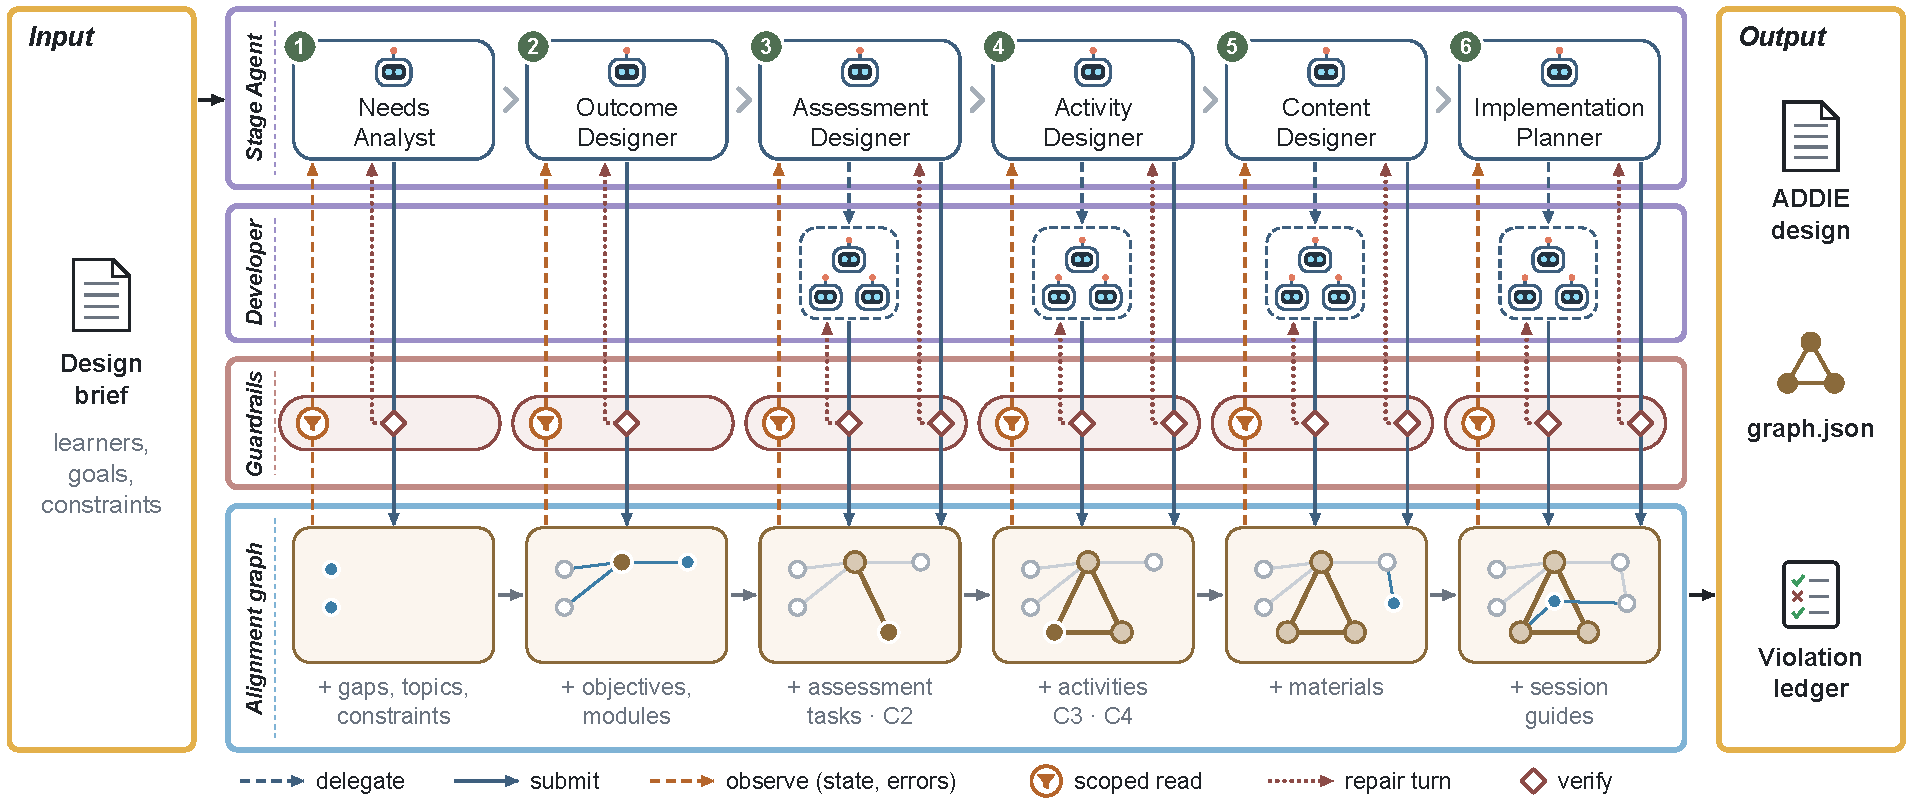
\includegraphics[width=\textwidth]{architecture_timeline.pdf}
  \caption{Kiến trúc AlignmentGraph-ISD. Sáu Stage Agent giữ lượt theo thứ tự 1--6;
  ở bốn giai đoạn, Developer viết các nhóm việc suy ra từ sản phẩm của Stage Agent.
  Mọi lượt đọc và nộp đi qua lớp kiểm soát (guardrails) của khung điều phối: lượt
  đọc chỉ trả về phạm vi của vai; lượt nộp đạt kiểm tra thì được ghi vào đồ thị,
  không đạt thì lỗi được trả về bên đã nộp để sửa. Hàng dưới cùng là đồ thị sau
  từng giai đoạn; tam giác C2--C4 khép lại ở giai đoạn 4.}
  \label{fig:arch}
\end{figure*}

Mỗi giai đoạn do một Stage Agent có vai riêng đảm nhận.
(1)~\emph{Phân tích nhu cầu} (Needs Analyst Agent): khoảng trống năng lực, hồ sơ người học, chủ đề và
ràng buộc. (2)~\emph{Mục tiêu và mô-đun} (Outcome Designer Agent): mục tiêu học tập và các mô-đun; mỗi mô-đun gom một số mục tiêu và chủ đề, kèm thời lượng. (3)~\emph{Đánh giá} (Assessment Designer Agent): kế
hoạch đánh giá với bảng đặc tả (blueprint) các nhiệm vụ đánh giá theo mô-đun;
mỗi nhiệm vụ có thời điểm (chẩn đoán, quá trình hoặc tổng kết), hình thức và quy
mô. (4)~\emph{Hoạt động} (Activity Designer Agent): chiến lược dạy học. (5)~\emph{Học liệu} (Content Designer Agent): lựa chọn
phương tiện. (6)~\emph{Triển khai} (Implementation Planner Agent): sáu sản phẩm gồm tập huấn giảng viên, kiểm
tra hệ thống, chạy thử, giám sát, tài liệu hướng dẫn giảng viên và tài liệu hướng
dẫn vận hành.

Thứ tự trên tuân theo thiết kế ngược (Backward Design): xác định kết quả mong
muốn trước, sau đó đến bằng chứng đánh giá và cuối cùng là kế hoạch học
tập~\cite{wiggins2005ubd}. Thứ tự này được chỉ thị trong prompt và cố định. Tác
tử tự chủ trong cách thực hiện một giai đoạn nhưng không chọn giai đoạn kế tiếp.
Vì vậy, hệ là một MAS phân rã theo vai kiểu quy trình (workflow-style). Hệ điều
phối tĩnh, không có thương lượng và không lập kế hoạch động giữa các
vai~\cite{hong2024metagpt}. Hệ không có giai đoạn riêng cho pha Evaluation của ADDIE. ADDIE là cấu
trúc của đầu ra: bộ tổng hợp (aggregator) sắp xếp nội dung từ đồ thị thành năm
pha theo định dạng mà benchmark yêu cầu.

\subsection{Đồ thị căn chỉnh}
\label{sec:graph}

Trạng thái dùng chung là một đồ thị có hướng
\begin{equation}
\label{eq:graph}
G=(V,E),\qquad E\subseteq V\times V\times\mathcal{R}.
\end{equation}
Mỗi nút $v\in V$ là một sản phẩm thiết kế có kiểu, như khoảng trống năng lực, chủ
đề, ràng buộc, hồ sơ người học, mục tiêu, mô-đun, nhiệm vụ đánh giá, hoạt động,
học liệu hay hướng dẫn buổi học. Mỗi cạnh $(u,v,r)$ nối hai sản phẩm qua một quan hệ $r$
thuộc tập $\mathcal{R}$ gồm 17 kiểu quan hệ. Ký hiệu $E_r=\{(u,v)\colon(u,v,r)\in E\}$.
Ba quan hệ cốt lõi là ba cạnh của tam giác căn chỉnh kiến tạo: $C_2$
(\texttt{assessed\_by}) nối mục tiêu với nhiệm vụ đánh giá đo nó, $C_3$
(\texttt{practiced\_by}) nối mục tiêu với hoạt động luyện tập nó, và $C_4$
(\texttt{prepares\_for}) nối hoạt động với nhiệm vụ đánh giá mà nó chuẩn bị. Mười
bốn quan hệ phụ $P_1$--$P_{14}$ ghi nguồn gốc, cách tổ chức theo mô-đun và việc
truy vết khi triển khai, ví dụ $P_{12}$ ghi mô-đun nào nhóm mục tiêu nào. Mô-đun
chỉ tham gia quan hệ phụ, vì nó tổ chức khóa học chứ không phải một đỉnh của tam
giác. Quan hệ phụ không được dùng làm bằng chứng về độ giá trị khái niệm (construct validity).

Một mục tiêu $o$ được căn chỉnh về cấu trúc khi tam giác khép kín trên nó:
\begin{equation}
\label{eq:aligned}
\begin{aligned}
\mathrm{aligned}(o)\iff\exists\,h,d\colon\;&(o,h)\in E_{C_3}\wedge(o,d)\in E_{C_2}\\
&\wedge(h,d)\in E_{C_4},
\end{aligned}
\end{equation}
trong đó $h$ là một hoạt động và $d$ là một nhiệm vụ đánh giá. Ba cạnh phải gặp
nhau trên cùng một hoạt động và cùng một nhiệm vụ. Ba điều kiện tồn tại tách rời
là chưa đủ, vì hoạt động có thể chuẩn bị cho một nhiệm vụ không đo $o$.

Với mỗi quan hệ $r$, gọi $S_r$ là tập nút thuộc phía phủ (coverage side) của $r$
và $N_r(v)$ là tập nút nối với $v$ qua $r$ theo hướng đó. Độ phủ của $r$ là
\begin{equation}
\label{eq:coverage}
\mathrm{cov}(r)=\frac{\bigl|\{v\in S_r\colon N_r(v)\neq\emptyset\}\bigr|}{|S_r|}.
\end{equation}
Ví dụ, $\mathrm{cov}(C_2)$ là tỉ lệ mục tiêu có ít nhất một nhiệm vụ đánh giá đo
nó. Điều kiện~\eqref{eq:aligned} và độ phủ~\eqref{eq:coverage} là đại lượng cấu
trúc: chúng cho biết quan hệ có tồn tại hay không, không cho biết thiết kế có giá
trị sư phạm hay không.

Cạnh không do mô hình tạo ra. Mỗi sản phẩm khai báo mã định danh (id) của các
sản phẩm mà nó phục vụ, ví dụ một hoạt động khai báo mục tiêu mà nó luyện tập.
Khi ghi sản phẩm, khung điều phối tra từng id và tự ghi cạnh có kiểu. Vì vậy,
quan hệ hình thành đúng tại thời điểm ghi. Một id không trỏ tới nút nào thì không
tạo cạnh. Phần thiếu hụt này được phản ánh trong độ phủ.

\subsection{Vòng lặp act--observe của một tác tử}
\label{sec:loop}

Mỗi tác tử chạy một vòng lặp hành động--quan sát (act--observe) theo mẫu
ReAct~\cite{yao2023react}, dùng cơ chế gọi công cụ (tool calling) gốc của mô hình. Công cụ
\texttt{read\_alignment\_state} không có tham số và trả về lát cắt đồ thị theo vai
của tác tử: những gì đã có kèm id, phần do tác tử viết, những gì còn thiếu mà sản
phẩm của nó phải bù, và các vi phạm đang mở của nó. Công cụ \texttt{read\_node}
trả về trọn một sản phẩm. Mỗi sản phẩm của giai đoạn có một công cụ nộp riêng
\texttt{submit\_<sản phẩm>}. Không có bước sinh riêng: sản phẩm chính là tham số
của lời gọi nộp. Mọi lượt đọc và nộp đều đi qua lớp kiểm soát của khung điều phối
(Hình~\ref{fig:arch}): lượt đọc chỉ trả về phạm vi của vai, và lượt đọc lặp lại
mà kết quả không đổi bị từ chối.

Khung điều phối kiểm tra mỗi lần nộp bằng bộ kiểm tra hợp lệ (validator) của sản
phẩm. Lần nộp hợp lệ được ghi thành nút có kiểu kèm các cạnh như ở
Mục~\ref{sec:graph}. Lần nộp không hợp lệ bị từ chối, và thông báo lỗi của
validator trở thành quan sát kế tiếp để tác tử sửa và nộp lại. Mỗi sản phẩm được nộp tối đa ba lần không tiến triển. Mỗi giai đoạn có trần số lượt. Nếu một giai đoạn không hoàn tất
trong các giới hạn này, khung điều phối vẫn ghi phần tốt nhất mà mô hình đã viết,
đánh dấu giai đoạn là bỏ dở (\texttt{gave\_up}) và báo cáo nó cùng kết quả.

Có bốn họ sản phẩm mà số lượng tăng theo quy mô thiết kế: câu hỏi đánh giá (nằm
trong nhiệm vụ đánh giá), hoạt động học tập, học liệu và hướng dẫn buổi học. Các
họ này do tầng tác tử phát triển (Developer) viết, mỗi Developer đảm nhận một
nhóm việc (work set). Nhóm việc được suy ra từ thiết kế đã có: mỗi mô-đun là một
nhóm, riêng họ đánh giá thì mỗi mục của bảng đặc tả là một nhóm. Mô hình không
tự chọn cách chia nhóm. Developer chạy cùng kiểu vòng lặp act--observe và
ghi vào cùng đồ thị. Nếu sau đó vẫn còn phần thiếu hụt, khung điều phối giao lại nhóm việc liên quan cho Developer, tối đa một lần, kèm danh sách những gì còn thiếu.

\subsection{Kiểm tra, sửa và sổ vi phạm}
\label{sec:repair}

Sau mỗi giai đoạn, khung điều phối chạy các phép kiểm tra tất định gắn với giai
đoạn đó mà không gọi mô hình. Các phép kiểm tra gồm: sự phù hợp giữa động từ
Bloom và mức nhận thức khai báo, tính đo được của mục tiêu, độ phủ quan hệ, tính
nhất quán của bảng đặc tả, tính đầy đủ của câu hỏi, mức thực hành chủ động, ngân
sách thời gian, việc xếp lịch cho hoạt động và học liệu, và tính khả thi.

Việc sửa có hai tầng. Tầng thứ nhất là sửa cấu trúc do khung điều phối thực hiện
mà không gọi mô hình. Tầng này chỉ sắp xếp lại những gì thiết kế đã có, ví dụ trỏ
lại một tham chiếu không hợp lệ hoặc thay động từ ngoài thang Bloom bằng động từ
mà mức khai báo cho phép. Tầng thứ hai dành cho vi phạm cần viết thêm nội dung.
Vi phạm loại này được trả về tác tử sở hữu thành một lượt sửa trong chính hội
thoại của tác tử đó. Tác tử đọc lại trạng thái, thấy vi phạm đang mở và nộp lại.
Khung điều phối không tự viết nội dung giảng dạy. Với một số loại vi phạm, khung điều phối không sửa mà chỉ báo cáo và đếm nếu còn tồn tại.

Mỗi vi phạm được ghi vào sổ vi phạm cùng kết cục: còn mở, do
khung điều phối sửa hoặc do tác tử sửa. Với vi phạm còn mở, sổ ghi lý do: tác tử
đã thấy nhưng không sửa được, hết ngân sách, không có tác tử nào sở hữu, hoặc chưa được đưa tới tác tử nào. Sau sáu giai đoạn, một lượt đối chiếu (reconciliation) tất
định gán các vi phạm liên giai đoạn còn lại cho tác tử sở hữu và chỉ sửa cấu trúc, không gọi mô hình. Bộ tổng hợp lắp đầu ra ADDIE từ đồ thị. Bộ kiểm toán ghi lại các vi phạm
còn tồn tại.

Mỗi lần chạy xuất ra hai tệp. Tệp \texttt{graph.json} chứa mọi nút, cạnh có kiểu
và các cạnh tam giác của từng mục tiêu. Tệp \texttt{violations.json} chứa sổ vi
phạm. Người thiết kế giảng dạy có thể truy vết từng quan hệ
mục tiêu--hoạt động--đánh giá và can thiệp khi cần, theo nguyên tắc giảng viên
trong vòng lặp (teacher-in-the-loop). Vì vậy, cơ chế kiểm tra--sửa đóng vai trò sửa dự phòng và cung cấp bằng chứng kiểm toán.

\section{THỰC NGHIỆM VÀ ĐÁNH GIÁ}
\label{sec:experiments}
% Khung đã chốt: Qwen3.5-2B, test_30, một lần chạy mỗi ô; TN1 = 7 hệ, TN2 = 2x2.
% Cấu hình: experiments/experiment.toml (dòng "# [full]" là bản đầy đủ). Mọi số sinh từ dữ liệu.

\subsection{Thiết lập thực nghiệm}
\label{sec:setup}

\subsubsection{Dữ liệu và mô hình}
Chúng tôi dùng 30 kịch bản thuộc tập kiểm tra của
ISD-Agent-Bench~\cite{isdagentbench}. Tập này tách biệt với 10 kịch bản đã dùng trong giai đoạn hoàn thiện hệ. Mọi hệ chạy trên cùng mô hình Qwen3.5-2B, vận hành tại chỗ bằng vLLM, với nhiệt độ sinh mặc định 0.7 (EduPlanner giữ nhiệt độ riêng cho từng vai theo thiết kế gốc) và cùng trần 8192 token cho mỗi lượt gọi. Phần suy luận của mô hình dùng chung ngân sách này và bị giới hạn ở 32 token; đây là trần chứ không phải tắt suy luận, được chốt trước khi chạy chính thức. Trần này là ngân sách mà một mô hình 4B để lại trên một GPU
12--16\,GB, tức môi trường triển khai mà bài báo nhắm tới. Mỗi ô (hệ, kịch bản)
được sinh một lần. Vì nhiệt độ sinh khác không, một lần sinh không phải là một
giá trị tất định. Khi một lượt nộp của hệ đề xuất bị từ chối, hệ viết lại sản phẩm
đó một lần bằng giải mã có ràng buộc (constrained decoding) theo JSON Schema của
sản phẩm. Đây là cơ chế sẵn có của vLLM, và điều kiện phục vụ này giống nhau ở mọi
biến thể của hệ. Hai lượt sinh của EduPlanner lỗi do mất kết nối tới máy chủ mô hình. Một kịch bản có tệp đầu vào sai tên trường, và tệp được sửa theo bản gốc của benchmark. Các ô này được sinh lại với cùng cấu hình trước khi chấm. Hệ đề xuất được sinh riêng ở mỗi thí nghiệm, nên số liệu của nó ở Bảng~\ref{tab:judge} và Bảng~\ref{tab:ablation} khác nhau đôi chút.

\subsubsection{Thí nghiệm 1 -- so sánh với các hệ của benchmark}
AlignmentGraph-ISD được so sánh với sáu tác tử của ISD-Agent-Bench trên cùng 30 kịch bản: Baseline (sinh một
lượt), React-ADDIE (kết hợp ADDIE với kiểu suy luận ReAct~\cite{yao2023react}),
ADDIE-Agent, Dick-Carey-Agent, RPISD-Agent và EduPlanner~\cite{zhang2025eduplanner}.
Tên tác tử theo bài báo gốc; prompt của React-ADDIE được dịch sang tiếng Anh, không đổi phương pháp.

\subsubsection{Thí nghiệm 2 -- phân tích thành phần}
Để tách vai trò của hai lựa chọn thiết kế, chúng tôi dùng thiết kế thực nghiệm
giai thừa $2\times2$. Trục \emph{phân rã} so sánh sáu tác tử theo vai (multi) với
một tác tử duy nhất duy trì một ngữ cảnh qua cả sáu giai đoạn (single). Trục
\emph{trạng thái} so sánh đồ thị căn chỉnh (graph) với một bảng chung (blackboard) dạng văn bản (prose). Trong biến thể prose, mỗi giai đoạn lưu nguyên văn sản phẩm và
giai đoạn sau đọc lại toàn văn. Mỗi trục là một gói cơ chế. Trục phân rã thay đổi cùng lúc ranh giới ngữ cảnh, số vai, tầng Developer, việc chia và giao lại nhóm việc, và thời điểm sửa. Trục trạng
thái thay đổi toàn bộ bộ máy căn chỉnh: đồ thị, công cụ đọc trạng thái, định tuyến
vi phạm và kiểm toán. Vì vậy, kết quả được diễn giải theo gói, không quy cho một
thành phần riêng lẻ.

\subsubsection{Điểm LLM judge}
Điểm ADDIE (0--100) đánh giá sản phẩm theo 33 tiêu chí con, gộp thành năm pha.
Điểm Trajectory đánh giá quá trình gọi công cụ. Điểm tổng hợp là
\begin{equation}
\label{eq:total}
\mathrm{Total}=0.7\cdot\mathrm{ADDIE}+0.3\cdot\mathrm{Trajectory}.
\end{equation}
Ba điểm được báo cáo song song. ADDIE là điểm dẫn vì nó đo chất lượng nội dung
thiết kế. Ba LLM judge của ba hãng khác nhau (GPT-6 Luna, Gemini~3.1 Flash-Lite, DeepSeek-V4.1-Flash) chấm mỗi đầu ra, với suy luận tắt. Điểm cuối cùng là trung vị của ba điểm. Không hãng nào trùng với hãng của mô hình tác tử. GPT-6 Luna không nhận tham số nhiệt độ nên không tất định. Bộ chấm của benchmark chỉ
đưa cho LLM judge 20 lời gọi công cụ đầu tiên. Do đó, hệ phân rã chịu bất lợi cơ
học ở điểm Trajectory.

\subsubsection{Tín hiệu căn chỉnh}
Vì LLM judge chấm từng pha riêng rẽ, chúng tôi đo thêm sáu tín hiệu liên quan đến
căn chỉnh kiến tạo trên chính đầu ra mà không dùng LLM. Họ A đo mức tương ứng văn
bản trên ba cạnh của tam giác: mục tiêu--đánh giá (OA), mục tiêu--hoạt động (OT)
và hoạt động--đánh giá (TA). Với mỗi phần tử nguồn, lấy cosine lớn nhất với các phần tử đích và cắt giá trị âm về 0; tín hiệu là trung bình các giá trị này (rectified cosine trên $[0,1]$). Phép đo không dùng ngưỡng ghép cặp. Văn bản được nhúng
bằng bge-m3. Họ B đo mức nhận thức theo thang phân loại Bloom sửa
đổi~\cite{anderson2001taxonomy}. Cg là tỉ lệ mục tiêu mà câu hỏi đánh giá gần nhất
với nó (theo cosine, không ngưỡng) có mức Bloom không thấp hơn mức của mục tiêu.
Vì dùng cosine để ghép cặp, Cg không hoàn toàn độc lập với họ A. Po là chỉ số Porter~\cite{porter2002measuring} trung bình trên ba cạnh của họ A. Wb là tính nhất quán mức nhận thức theo Webb~\cite{webb1997criteria}, xét từ phía từng câu hỏi. Mức Bloom được gán bằng một bộ phân loại BERT tinh
chỉnh trên dữ liệu mục tiêu học tập và câu hỏi thi do chuyên gia gán nhãn. Tín
hiệu bằng 0 khi hệ không sinh ra tập phần tử tương ứng. Quy trình chấm không dùng
LLM và không có thành phần ngẫu nhiên. Kết quả tái lập được, sai khác chỉ ở mức
nhiễu dấu phẩy động, nhờ cố định phiên bản encoder và lưu đệm embedding. Các tín hiệu này chỉ phản ánh một số khía cạnh đo được của căn chỉnh kiến tạo.

\subsubsection{Thước đo quá trình và thống kê}
Với Thí nghiệm~2, chúng tôi tính tỉ lệ mục tiêu có đủ ba cạnh $C_2$, $C_3$, $C_4$ theo~\eqref{eq:aligned} trên đầu ra của cả bốn biến thể. Thước đo này tính được trên cả đồ thị lẫn bảng chung. Đây là mức tuân thủ cấu trúc, không
phải giá trị sư phạm. Các bảng ghi trung bình qua 30 kịch bản; Bảng~\ref{tab:judge} và cột ADDIE của Bảng~\ref{tab:ablation} ghi thêm độ lệch chuẩn. Ở Thí nghiệm~1, hệ đề xuất được so sánh với từng hệ còn lại bằng kiểm định
Wilcoxon theo cặp kịch bản. Giá trị $p$ được hiệu chỉnh Holm trong từng điểm số
hoặc từng tín hiệu. Ở Thí nghiệm~2, hai kiểm định được đăng ký trước khi chạy chính thức, với giả thuyết multi cao hơn single về điểm ADDIE và graph cao hơn prose về tỉ lệ mục tiêu khép kín tam giác. Thước đo của trục trạng thái được chốt sau khi xem dữ liệu của giai đoạn hoàn thiện, trước khi chạy chính thức. Hai kiểm định này thuộc cùng một họ hiệu chỉnh Holm.
Ở cả hai thí nghiệm, hệ không sinh ra đầu ra chấm được ở một kịch bản thì nhận
0 điểm ở kịch bản đó. Điểm LLM judge là số rời rạc. Vì vậy, chênh lệch theo cặp thường có
hạng trùng hoặc bằng 0. Giá trị $p$ của Wilcoxon được tính chính xác theo phân phối hoán vị có điều kiện (conditional permutation), dùng thuật toán shift~\cite{streitberg1986exact}.
Khoảng tin cậy bootstrap được tính bằng SciPy~\cite{virtanen2020scipy}.

\subsection{Kết quả}
\label{sec:results}

% Bảng I: TN1, điểm LLM judge + chi phí. Sinh bằng script, không gõ tay.
\IfFileExists{generated/tab_judge.tex}{\begin{table}[t]
  \caption{Thí nghiệm 1: điểm LLM judge (trung bình $\pm$ độ lệch chuẩn qua 30 kịch bản) và token mỗi kịch bản}
  \label{tab:judge}
  \centering
  \footnotesize
  \setlength{\tabcolsep}{2.5pt}
  \begin{tabular}{@{}lcccc@{}}
    \toprule
    Hệ & ADDIE $\uparrow$ & Trajectory $\uparrow$ & Total $\uparrow$ & Token (k) $\downarrow$ \\
    \midrule
    AlignmentGraph-ISD & 59.0\,$\pm$\,2.8 & 69.7\,$\pm$\,5.9 & 62.2\,$\pm$\,2.3 & 282 \\
    EduPlanner & 30.0\,$\pm$\,19.8$^{*}$ & 53.0\,$\pm$\,32.7 & 36.9\,$\pm$\,23.2$^{*}$ & 70 \\
    Baseline & 43.4\,$\pm$\,17.7$^{*}$ & 69.2\,$\pm$\,19.0 & 51.1\,$\pm$\,16.6$^{*}$ & 10 \\
    React-ADDIE & \textbf{59.1\,$\pm$\,6.7} & 71.5\,$\pm$\,9.5 & \textbf{62.8\,$\pm$\,4.9} & 15 \\
    ADDIE-Agent & 48.5\,$\pm$\,3.6$^{*}$ & \textbf{81.5\,$\pm$\,3.0$^{*}$} & 58.4\,$\pm$\,2.7$^{*}$ & 23 \\
    Dick-Carey-Agent & 58.0\,$\pm$\,3.0 & 72.6\,$\pm$\,5.6 & 62.4\,$\pm$\,3.1 & 26 \\
    RPISD-Agent & 58.4\,$\pm$\,2.5 & 69.9\,$\pm$\,3.3 & 61.8\,$\pm$\,1.9 & 61 \\
    \bottomrule
  \end{tabular}
  \par\vspace{2pt}
  {\scriptsize\raggedright $^{*}$ khác AlignmentGraph-ISD, Wilcoxon theo cặp, Holm trong từng điểm, $p<0.05$.\\ Kịch bản không có đầu ra chấm được, tính 0 điểm: EduPlanner 8, Baseline 2.\par}
\end{table}
}{%
\begin{table}[t]
  \caption{Thí nghiệm 1: điểm LLM judge và chi phí trên 30 kịch bản}
  \label{tab:judge}
  \centering
  \footnotesize
  \setlength{\tabcolsep}{4pt}
  \begin{tabular}{@{}lcccc@{}}
    \toprule
    Hệ & ADDIE $\uparrow$ & Trajectory $\uparrow$ & Total $\uparrow$ & Token (k) \\
    \midrule
    AlignmentGraph-ISD & \TBD & \TBD & \TBD & \TBD \\
    Baseline & \TBD & \TBD & \TBD & \TBD \\
    React-ADDIE & \TBD & \TBD & \TBD & \TBD \\
    ADDIE-Agent & \TBD & \TBD & \TBD & \TBD \\
    Dick-Carey-Agent & \TBD & \TBD & \TBD & \TBD \\
    RPISD-Agent & \TBD & \TBD & \TBD & \TBD \\
    EduPlanner & \TBD & \TBD & \TBD & \TBD \\
    \bottomrule
  \end{tabular}
\end{table}}

% Bảng II: TN1, sáu tín hiệu căn chỉnh.
\IfFileExists{generated/tab_panel.tex}{\begin{table}[t]
  \caption{Thí nghiệm 1: tín hiệu căn chỉnh (trung bình qua 30 kịch bản)}
  \label{tab:panel}
  \centering
  \footnotesize
  \setlength{\tabcolsep}{3pt}
  \begin{tabular}{@{}lcccccc@{}}
    \toprule
    & \multicolumn{3}{c}{Họ A: văn bản} & \multicolumn{3}{c}{Họ B: Bloom} \\
    \cmidrule(lr){2-4}\cmidrule(l){5-7}
    Hệ & OA $\uparrow$ & OT $\uparrow$ & TA $\uparrow$ & Cg $\uparrow$ & Po $\uparrow$ & Wb $\uparrow$ \\
    \midrule
    AlignmentGraph-ISD & \textbf{0.76} & \textbf{0.75} & \textbf{0.71} & 0.75 & \textbf{0.42} & 0.66 \\
    EduPlanner & 0.43$^{*}$ & 0.40$^{*}$ & 0.35$^{*}$ & 0.45$^{*}$ & 0.17$^{*}$ & 0.40$^{*}$ \\
    Baseline & 0.45$^{*}$ & 0.33$^{*}$ & 0.29$^{*}$ & 0.57 & 0.13$^{*}$ & 0.45$^{*}$ \\
    React-ADDIE & 0.69$^{*}$ & 0.63$^{*}$ & 0.57$^{*}$ & 0.68 & 0.22$^{*}$ & 0.52$^{*}$ \\
    ADDIE-Agent & 0.69$^{*}$ & 0.64$^{*}$ & 0.52$^{*}$ & 0.69 & 0.30$^{*}$ & 0.58 \\
    Dick-Carey-Agent & 0.66$^{*}$ & 0.63$^{*}$ & 0.62$^{*}$ & \textbf{0.78} & 0.34$^{*}$ & \textbf{0.69} \\
    RPISD-Agent & 0.64$^{*}$ & 0.65$^{*}$ & 0.52$^{*}$ & 0.53$^{*}$ & 0.28$^{*}$ & 0.50$^{*}$ \\
    \bottomrule
  \end{tabular}
  \par\vspace{2pt}
  {\scriptsize\raggedright $^{*}$ khác AlignmentGraph-ISD, Wilcoxon theo cặp, Holm trong từng tín hiệu, $p<0.05$.\par}
\end{table}
}{%
\begin{table}[t]
  \caption{Thí nghiệm 1: tín hiệu căn chỉnh (trung bình trên 30 kịch bản)}
  \label{tab:panel}
  \centering
  \footnotesize
  \setlength{\tabcolsep}{4pt}
  \begin{tabular}{@{}lcccccc@{}}
    \toprule
    & \multicolumn{3}{c}{Họ A: văn bản} & \multicolumn{3}{c}{Họ B: Bloom} \\
    \cmidrule(lr){2-4}\cmidrule(l){5-7}
    Hệ & OA $\uparrow$ & OT $\uparrow$ & TA $\uparrow$ & Cg $\uparrow$ & Po $\uparrow$ & Wb $\uparrow$ \\
    \midrule
    AlignmentGraph-ISD & \TBD & \TBD & \TBD & \TBD & \TBD & \TBD \\
    Baseline & \TBD & \TBD & \TBD & \TBD & \TBD & \TBD \\
    React-ADDIE & \TBD & \TBD & \TBD & \TBD & \TBD & \TBD \\
    ADDIE-Agent & \TBD & \TBD & \TBD & \TBD & \TBD & \TBD \\
    Dick-Carey-Agent & \TBD & \TBD & \TBD & \TBD & \TBD & \TBD \\
    RPISD-Agent & \TBD & \TBD & \TBD & \TBD & \TBD & \TBD \\
    EduPlanner & \TBD & \TBD & \TBD & \TBD & \TBD & \TBD \\
    \bottomrule
  \end{tabular}
\end{table}}

% Bảng III: TN2, 2x2.
\IfFileExists{generated/tab_ablation.tex}{\begin{table}[t]
  \caption{Thí nghiệm 2: phân rã $\times$ trạng thái (30 kịch bản)}
  \label{tab:ablation}
  \centering
  \footnotesize
  \setlength{\tabcolsep}{3pt}
  \begin{tabular}{@{}lcccc@{}}
    \toprule
    Biến thể & ADDIE $\uparrow$ & Total $\uparrow$ & Khép kín (\%) $\uparrow$ & Token (k) $\downarrow$ \\
    \midrule
    multi, graph (đề xuất) & 58.2\,$\pm$\,2.6 & 62.4 & 86 & 278 \\
    multi, prose & \textbf{58.6\,$\pm$\,2.6} & \textbf{64.1} & \textbf{87} & 255 \\
    single, graph & 53.1\,$\pm$\,3.7 & 56.5 & 67 & 428 \\
    single, prose & 53.9\,$\pm$\,3.0 & 56.7 & 69 & 414 \\
    \bottomrule
  \end{tabular}
  \par\vspace{2pt}
  {\scriptsize\raggedright Khép kín: tỉ lệ mục tiêu có đủ ba cạnh $C_2$--$C_4$ trong đầu ra.\par}
\end{table}
}{%
\begin{table}[t]
  \caption{Thí nghiệm 2: phân rã $\times$ trạng thái}
  \label{tab:ablation}
  \centering
  \footnotesize
  \setlength{\tabcolsep}{3pt}
  \begin{tabular}{@{}lcccc@{}}
    \toprule
    Biến thể & ADDIE $\uparrow$ & Total $\uparrow$ & Khép kín (\%) $\uparrow$ & Token (k) \\
    \midrule
    multi, graph (đề xuất) & \TBD & \TBD & \TBD & \TBD \\
    multi, prose & \TBD & \TBD & \TBD & \TBD \\
    single, graph & \TBD & \TBD & \TBD & \TBD \\
    single, prose & \TBD & \TBD & \TBD & \TBD \\
    \bottomrule
  \end{tabular}
\end{table}}

\subsubsection{Thí nghiệm 1}
Bảng~\ref{tab:judge} trình bày điểm LLM judge. Về điểm ADDIE, AlignmentGraph-ISD
(\cmpAGAddie) không khác biệt có ý nghĩa với React-ADDIE (\cmpReactAddie,
$p$\,\cmpReactAddieP), Dick-Carey-Agent (\cmpDickAddie) và RPISD-Agent
(\cmpRpisdAddie). Hệ đề xuất cao hơn ADDIE-Agent \cmpAddieAddieDiff{} điểm,
Baseline \cmpBaseAddieDiff{} điểm và EduPlanner \cmpEduAddieDiff{} điểm
($p$\,\cmpEduAddieP{} ở cả ba so sánh). Một phần chênh lệch với hai hệ sau đến từ các kịch bản không
có đầu ra chấm được (chú thích Bảng~\ref{tab:judge}). Baseline hỏng vì đầu ra chạm
trần 8192 token, còn EduPlanner hỏng vì đầu ra không khớp schema của chính nó. Về
điểm Trajectory, ADDIE-Agent đạt cao nhất (\cmpAddieTraj) và cao hơn có ý nghĩa so với hệ đề xuất ($p$\,\cmpAddieTrajP). Về điểm Total, hệ đề xuất không khác biệt có ý nghĩa với React-ADDIE, Dick-Carey-Agent và RPISD-Agent.

Bảng~\ref{tab:panel} trình bày sáu tín hiệu căn chỉnh. AlignmentGraph-ISD có ba tín
hiệu họ A cao nhất (OA \panAGOA, OT \panAGOT, TA \panAGTA) và chỉ số Porter cao
nhất (\panAGPo). Các khác biệt này có ý nghĩa với cả sáu tác tử. Với Cg và Wb,
Dick-Carey-Agent đạt giá trị cao hơn hệ đề xuất nhưng khác biệt không có ý nghĩa
(Cg $p$\,\panDickCgP, Wb $p$\,\panDickWbP).

\subsubsection{Thí nghiệm 2}
Bảng~\ref{tab:ablation} trình bày bốn biến thể. Kiểm định đăng ký cho trục phân rã
ủng hộ giả thuyết: biến thể multi cao hơn single \ablHDDiff{} điểm ADDIE (khoảng
tin cậy 95\% [\ablHDCILo; \ablHDCIHi], $p$\,\ablHDP). Tỉ lệ mục tiêu khép kín tam
giác cũng tăng từ \ablSGTriad--\ablSPTriad\% ở biến thể single lên
\ablMGTriad--\ablMPTriad\% ở biến thể multi. Kiểm định đăng ký cho trục trạng thái
không phát hiện khác biệt: chênh lệch tỉ lệ khép kín của graph so với prose là $\ablHSDiff$ điểm phần trăm (khoảng tin cậy 95\% [$\ablHSCILo$; $\ablHSCIHi$],
$p$\,\ablHSP). Biến thể single tốn nhiều token hơn multi (\ablSGTok{}k so với
\ablMGTok{}k ở biến thể graph).

AlignmentGraph-ISD dùng trung bình \cmpAGTok{}k token cho mỗi kịch bản, khoảng
\cmpTokRatioReact{} lần React-ADDIE. Hệ có chi phí tính toán cao hơn đáng kể so với các hệ dạng quy
trình gọn nhẹ. Chúng tôi báo cáo chi phí này bên cạnh các tín hiệu căn chỉnh, khả
năng truy vết và khả năng kiểm toán, mà không diễn giải rằng hệ hiệu quả hơn về
mặt tính toán.

\subsection{Thảo luận}
\label{sec:discussion}

\textbf{(1) Cạnh tranh về điểm LLM judge.} Với mô hình 2B, điểm ADDIE của hệ đề xuất không khác biệt có ý nghĩa với các tác tử mạnh nhất của benchmark. Độ lệch chuẩn qua
kịch bản của hệ (\cmpAGAddieSD) thấp hơn React-ADDIE (\cmpReactAddieSD), tức điểm ADDIE ít dao động hơn giữa các kịch bản.

\textbf{(2) Tín hiệu họ A tách hệ đề xuất khỏi các tác tử mạnh, điểm ADDIE thì không.} Có hai cách đọc
kết quả này. Cách thứ nhất: LLM judge chấm từng pha ADDIE riêng rẽ nên không thấy
liên kết giữa các pha, đúng là lý do cần đo thêm tín hiệu căn chỉnh. Cách thứ hai: khung điều phối đã kiểm tra ngay lúc nộp một phần các ràng buộc mà các tín hiệu này đo, nên tín hiệu cao một phần phản ánh việc hệ tuân thủ ràng buộc của chính nó.
Bằng chứng độc lập cần đến đánh giá của chuyên gia.

\textbf{(3) Gói phân rã đa tác tử có tác dụng rõ với Qwen3.5-2B.} Gói này gồm các thay đổi nêu ở phần thiết lập Thí nghiệm~2. Với mô hình 2B, cả điểm ADDIE và
tỉ lệ khép kín tam giác đều tăng, đồng thời số token giảm.

\textbf{(4) Gói trạng thái đồ thị không tạo khác biệt đo được.} Biến thể prose không khác biệt có ý nghĩa so với graph về tỉ lệ khép kín, và điểm ADDIE của hai biến thể gần nhau. Trong thực nghiệm này, khác biệt của biến thể graph là hồ sơ kiểm toán mà biến thể prose không có.

\textbf{Hạn chế.} Thực nghiệm dùng một nấc mô hình, 30 kịch bản và một lần sinh cho
mỗi ô. Điểm LLM judge có thiên lệch. Chúng tôi dùng ba LLM judge thay cho cặp LLM
judge mặc định của benchmark. Các LLM judge này lệch nhau đáng kể về mức điểm tuyệt
đối, và thứ hạng giữa hệ đề xuất và React-ADDIE thay đổi theo từng LLM judge. Chúng
tôi đã kiểm tra rằng cả ba LLM judge nhận đủ các đầu ra dài và không chấm nội dung
có thật thành vắng mặt. Bằng chứng độc lập về chất lượng thiết kế cần đến đánh giá
của chuyên gia thiết kế giảng dạy. Kết quả được quan sát trên Qwen3.5-2B và chưa
được kiểm chứng trên các cỡ mô hình và các họ mô hình khác.

\section{KẾT LUẬN}
\label{sec:conclusion}
% Tóm tắt -- kết quả chính -- hướng phát triển. Không đưa claim mới.
Bài báo đã trình bày AlignmentGraph-ISD, một hệ đa tác tử phân rã theo vai cho
thiết kế giảng dạy. Trong hệ này, các tác tử dùng chung một đồ thị căn chỉnh làm
trạng thái trung tâm. Trên \NScenCmp{} kịch bản với Qwen3.5-2B, hệ đạt điểm LLM judge cạnh tranh với các tác tử mạnh nhất của benchmark và có các tín hiệu tương ứng văn bản cao hơn. Gói phân rã đa tác tử có tác dụng rõ trong thí nghiệm phân tích thành phần. Gói trạng thái đồ thị không tạo khác biệt về tỉ lệ khép kín, nhưng đồ thị cung cấp hồ sơ kiểm toán cho từng quan hệ
mục tiêu--hoạt động--đánh giá. Hướng phát triển gồm đánh giá trên nhiều cỡ mô hình,
lặp lại nhiều lần sinh cho mỗi kịch bản và lấy đánh giá của chuyên gia thiết kế
giảng dạy trên đồ thị và sổ vi phạm mà hệ xuất ra.

\bibliographystyle{IEEEtran}
\bibliography{refs}

\end{document}
